\section*{Exercise 3: Edge Detection Using FFT}

\subsection*{Problem Statement}
In image processing, besides other methods, the FFT can be utilized to conduct edge detection. To this end, a two-dimensional FFT (MATLAB command: `fft2`) is calculated from an image to transform it from the spatial domain to the frequency domain. Here, edges in an image produce high frequencies in the corresponding spectrum.

In this exercise, you should make the edges of an image visible. Start by making yourself familiar with the MATLAB script `fft_edge_detection`. Now filter the image in the frequency domain, such that the edges become visible after a transformation back to the spatial domain. Describe your approach and justify why it works. A solution could look like the one depicted in Fig. 1.

\subsection*{Python Script}
\begin{verbatim}
import numpy as np
import matplotlib.pyplot as plt
from scipy.fft import fft2, ifft2, fftshift
from imageio import imread

# Read the image
image_path = 'image.png'
image = imread(image_path, mode='L')

# Perform the 2D FFT
image_fft = fft2(image)
image_fft_shifted = fftshift(image_fft)  # Shift the zero frequency component to the center

# Create a high-pass filter
rows, cols = image.shape
crow, ccol = rows // 2 , cols // 2  # Center of the image

# Create a mask with high value at edges
high_pass_mask = np.ones((rows, cols), dtype=np.float32)
high_pass_radius = 30  # Adjust the radius to control the filter size
center_radius = high_pass_radius

for i in range(rows):
    for j in range(cols):
        if np.sqrt((i - crow)**2 + (j - ccol)**2) < center_radius:
            high_pass_mask[i, j] = 0

# Apply the high-pass filter
filtered_fft = image_fft_shifted * high_pass_mask

# Inverse FFT to transform back to the spatial domain
filtered_fft_shifted_back = fftshift(filtered_fft)
image_filtered = np.abs(ifft2(filtered_fft_shifted_back))

# Plot the original and filtered images
plt.figure(figsize=(12, 6))

plt.subplot(1, 2, 1)
plt.imshow(image, cmap='gray')
plt.title('Original Image')
plt.axis('off')

plt.subplot(1, 2, 2)
plt.imshow(image_filtered, cmap='gray')
plt.title('Edge Detection using FFT')
plt.axis('off')

# Save the plot for LaTeX inclusion
plt.savefig('fig/ex3_edge_detection_fft.png')
plt.show()
\end{verbatim}

\subsection*{Edge Detection using FFT}
\begin{figure}[h]
    \centering
    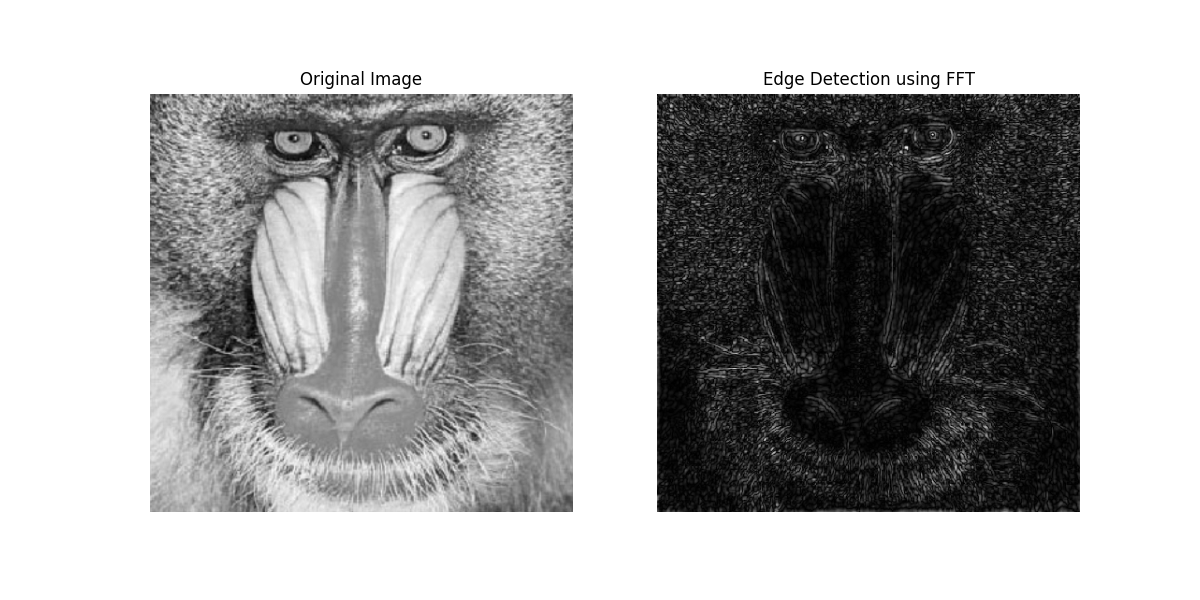
\includegraphics[width=0.8\textwidth]{fig/ex3_edge_detection_fft.png}
    \caption{Edge Detection using FFT}
    \label{fig:ex3_edge_detection_fft}
\end{figure}

\subsection*{Approach and Justification}
The approach involves the following steps:
\begin{enumerate}
    \item Perform a 2D FFT on the image to transform it from the spatial domain to the frequency domain.
    \item Apply a high-pass filter in the frequency domain to retain high-frequency components (which correspond to edges) and suppress low-frequency components (which correspond to smooth regions).
    \item Perform an inverse FFT to transform the filtered image back to the spatial domain.

This approach works because edges in an image correspond to abrupt changes in intensity, which translate to high frequencies in the frequency domain. By applying a high-pass filter, we can isolate these high-frequency components, making the edges visible in the spatial domain after the inverse FFT.
